\chapter{Results}
\label{ch:results}
\thispagestyle{fancy}

All the data preparation, analysis and visualization was done using the statistical software \textit{R} \citep{rcoreteam2014}\footnote{and the packages \textit{dplyr} \citep{wickham2017}, }. 
All data and scripts are available at XXX.XXX.XXX

\section{Descriptive Statistics and General Results}

Participants solved an average of 11.5 sequences in the competition rounds and spent an average of 85.2 seconds in the \textit{switch} mode. There was little difference in production between wages, i.e. between winners and losers, but some difference can be observed between treatments. Subjects in the treatment produced less in average and spent more time in the \textit{switch} mode. Table \ref{tab:avg_prod} and graph \ref{fig:production_boxplot} summarize these findings.\\

\begin{table}[!htbp] \centering
  \caption{Mean Values of Production\\
    \footnotesize{standard errors are reported in parentheses ()}} 
  \label{tab:avg_prod}
\begin{tabular}{@{\extracolsep{5pt}} cccc} 
\\[-1.8ex]\hline 
\hline \\[-1.8ex] 
treatment & wage & mean solved sequences & mean of time spent in switch \\ 
\hline \\[-1.8ex] 
0 & 1 & 12.02 & 78.66 \\ 
 &  & (0.23) & (3.13) \\ 
0 & 2 & 11.91 & 79.09 \\
 &  & (0.3) & (4.22) \\ 
1 & 1 & 11.1 & 92.28 \\
 &  & (0.21) & (2.86) \\ 
1 & 2 & 11.12 & 90.23 \\
 &  & (0.33) & (4.42) \\ 
\hline \\[-1.8ex]
\end{tabular}
\end{table}  

\begin{figure}
    \centering
    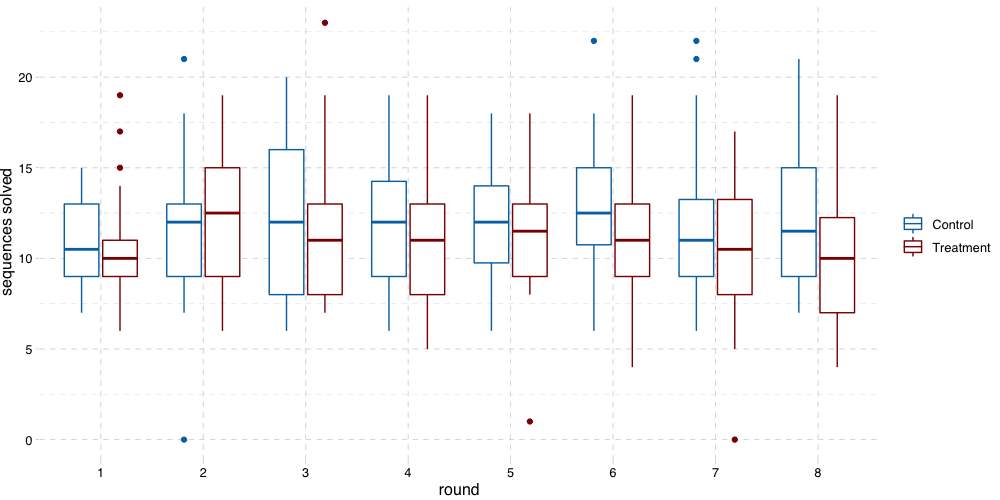
\includegraphics[width=\textwidth]{graphs/production_boxplot.png}
    \caption{Number of Sequences Solved per Round and Treatment}
    \label{fig:production_boxplot}
\end{figure}

\subsection{Sequence Production \& Income}
To see if the difference in production between the treatments is statistically significant, and to see how other factors play a role, I used a linear mixed model with random intercepts evaluated using the \textit{R} package \textit{lmer} \citep{bates2015}. I chose this model since it offers more flexibility than a traditional ANOVA analysis. Specially important for my design is the fact that it allows to have a random intercept for each subject and nesting in the group, since we might expect that certain participants tend to work and invest more than others and that that affects the overall performance of the group. Since the design allows only for between-groups comparisons regarding the treatment, I exclude a random slope per participant, assuming thus that the effect of time will be equivalent for all subjects.\\

In this model, the fixed effects are the \textit{treatment}, \textit{was winner} (if a participant won the previous round and is playing with the high wage), and the \textit{round} number. The random effect is the \textit{subjects id} nested within the \textit{group}. Results are reported following largely \cite{barr2013} and are summarized in table \ref{table:lmer_prod}. P-values were calculated using the likelihood ratio test.\\

The residual plot and qq-plot do not make apparent any deviation from a normal distribution nor any systematic increase or decrease in variance. \textit{Treatment} has a small although significant effect at the 0.1 level with subjects in the control group solving just shy of 1 sequence more. All the other fixed effects have no significant or large effect with the model in total explaining 42\% of the observed variance (conditional R-squared) in which the fixed effects explain 1.52\% (marginal r-squared). This includes, interestingly, the wage at which participants played.\\

\begin{table}[!htbp] \centering 
  \caption{Linear Mixed Model - Sequence Production} 
  \label{table:lmer_prod} 
  \scalebox{0.8}{%
\begin{tabular}{@{\extracolsep{5pt}}lc} 
\\[-1.8ex]\hline 
\hline \\[-1.8ex] 
 & \multicolumn{1}{c}{\textit{Dependent variable:}} \\ 
\cline{2-2} 
\\[-1.8ex] & Sequence Production \\ 
\hline \\[-1.8ex] 
 treatment & $-$0.872$^{*}$ \\ 
  & (0.499) \\ 
  & \\ 
 was winner & 0.028 \\ 
  & (0.231) \\ 
  & \\ 
 round & $-$0.003 \\ 
  & (0.043) \\ 
  & \\ 
 Constant & 11.985$^{***}$ \\ 
  & (0.408) \\ 
  & \\ 
\hline \\[-1.8ex] 
Observations & 768 \\ 
Log Likelihood & $-$1,943.528 \\ 
Akaike Inf. Crit. & 3,901.055 \\ 
Bayesian Inf. Crit. & 3,933.525 \\
\hline \\ [-1.8ex] 
Var: participant|group (Intercept) & 5.08\\
Var: group (Intercept) & 0.00 \\
Var: Residual & 7.28 \\
\hline \\[-1.8ex] 
\hline 
\textit{Note:}  & \multicolumn{1}{r}{$^{*}$p$<$0.1; $^{**}$p$<$0.05; $^{***}$p$<$0.01} \\ 
\end{tabular}
}
\end{table} 

In this experimental design, earnings are not exclusively determined by the amount of sequences solved. It depends also on time spent in the \textit{switch} mode and therefore on the optimal change to it; the invested amount and, in the treatment, how much the other players worked. The boxplot in figure \ref{fig:earnings_boxplot} seems to suggest that net income is higher in the treatment groups and that, apart from round 1, they do not change over time. Note that net income describes here income after taxation AND redistribution but before investment. To see if there were differences are significant, I use a model similar to the one explained above. With fixed effects \textit{treatment, was winner} and \textit{round}. Table \ref{table:earnings_lmer} summarizes the findings.\\

Winning the previous round, i.e. playing with the high wage has a strong and significant effect on net income while time, although slightly significant, has only a small effect. The introduction of a tax and redistribution, on the other hand, does not have a significant effect. The model helps explaining 50.11\% (restricted r-squared) of the variance with the fixed effects accounting for 33.73\% (marginal r-squared) of the variance. The residual plot and qq-plot do not make apparent any deviation from a normal distribution nor any systematic increase or decrease in variance.\\

A discussion about why the treatment fails to show an impact on net income is well beyond the scope of this thesis but it is addressed in the \textit{further research} section in chapter \ref{ch:conclusion}.


\begin{figure}
    \centering
    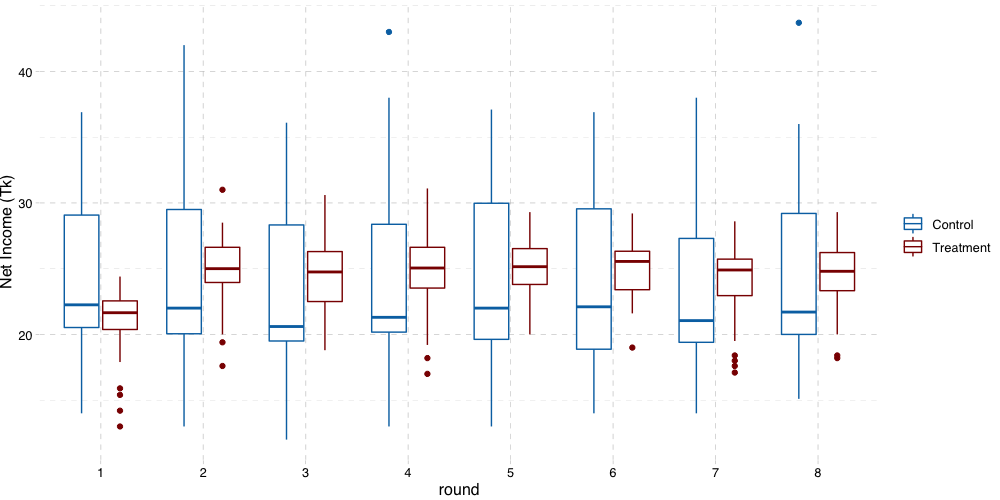
\includegraphics[width=\textwidth]{graphs/earnings_boxplot.png}
    \caption{Income after Taxation and Redistribution, and before investment}
    \label{fig:earnings_boxplot}
\end{figure}


\begin{table}[!htbp] \centering 
  \caption{Linear Mixed Model - Net Income} 
  \label{table:earnings_lmer}
  \scalebox{0.8}{%
\begin{tabular}{@{\extracolsep{5pt}}lc} 
\\[-1.8ex]\hline 
\hline \\[-1.8ex] 
 & \multicolumn{1}{c}{\textit{Dependent variable:}} \\ 
\cline{2-2} 
\\[-1.8ex] & net income \\ 
\hline \\[-1.8ex] 
 treatment & 0.598 \\ 
  & (0.471) \\ 
  & \\ 
 was winner & 5.977$^{***}$ \\ 
  & (0.289) \\ 
  & \\ 
 round & 0.090$^{*}$ \\ 
  & (0.054) \\ 
  & \\ 
 Constant & 21.434$^{***}$ \\ 
  & (0.422) \\ 
  & \\ 
\hline \\[-1.8ex] 
Observations & 768 \\ 
Log Likelihood & $-$2,098.867 \\ 
Akaike Inf. Crit. & 4,211.735 \\ 
Bayesian Inf. Crit. & 4,244.241 \\ 
\hline 
Var: participant|group (Intercept) & 3.86          \\
Var: group (Intercept)           & 0.00          \\
Var: Residual                              & 11.77         \\
\hline
\hline \\[-1.8ex] 
\textit{Note:}  & \multicolumn{1}{r}{$^{*}$p$<$0.1; $^{**}$p$<$0.05; $^{***}$p$<$0.01} \\ 
\end{tabular}
}
\end{table} 


\subsection{Optimum of Work Supply}
During the competition, participants tend to work more than their optimum, but decreasingly so with each round. Remember, participants should switch as soon as the time they need to solve a given task surpasses the earnings in the switch mode for the corresponding time. In the control group, players with the low wage should change as soon as they take longer than 10 seconds to solve the task, in the treatment, as soon as they need more than six seconds. In each treatment, players with the high wage should switch at twice the time. Graph X shows the time needed for each task per round and marks the 10 and 20 seconds cutoffs.\\ 

\begin{figure}
    \centering
    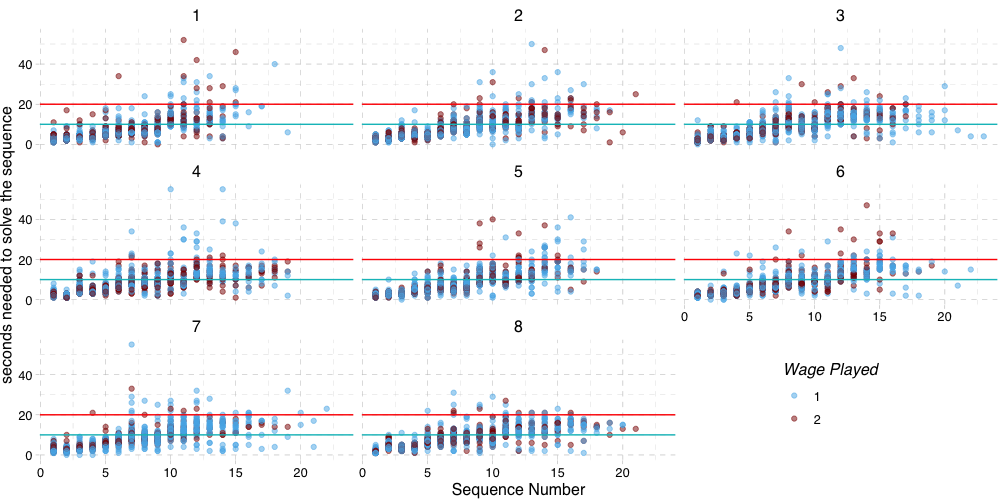
\includegraphics[width=\textwidth]{graphs/time_per_task.png}
    \caption{Count of Choice of Switching Row}
    \label{fig:time_per_task}
\end{figure}

Valuation avg \\

\subsection{Cognitive Reflection Test}
In the \textit{Cognitive Reflection Test}, participants answered, out of 4, in average 2.22 (s.e. 0.1) questions correctly. Men answered in average 0.3 (s.e. 0.15) more questions correctly with women giving 2.09 (s.e. 0.13) right answers in average.\\


\subsection{Risk Elicitation Task}
In the \textit{Risk Elicitation} task, participants chose in average row 6.6 to switch which according to table \ref{table:HL} indicates a risk averse to very risk averse behaviour. Men generally showed a more risk averse behaviour, switching in average at row 6.93 (s.e. 0.32), while women switched in average already at row 6.36 (s.e. 0.33). Figure \ref{fig:hist_mpl} shows a histogram of the row at which participants switched.\\

\begin{figure}
    \centering
    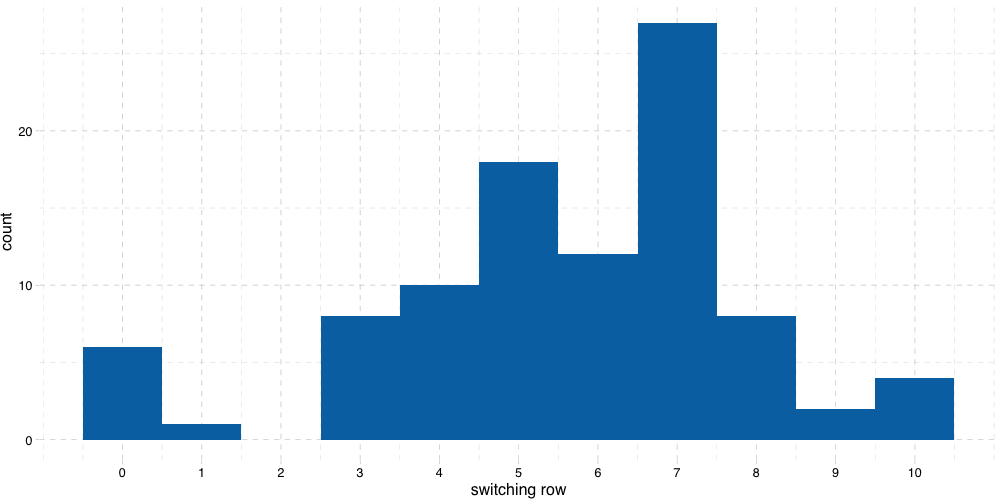
\includegraphics[width=\textwidth]{graphs/hist_mpl.png}
    \caption{Count of Choice of Switching Row}
    \label{fig:hist_mpl}
\end{figure}


\subsection{Hypothesis 1}

Since the treatment and control groups have different valuations, I analyze rather the mean difference over optimal investment for both groups. The optimal Investment is calculated on the assumption that participants have the same valuation, which is supported by a t-test.\\

Consistent with expectations, participants bid significantly more than their optimum but decreasingly so over time. Interestingly, participants in the taxation treatment invest both nominally and relatively more than those in the control, with treatment participants bidding in average 5 and a half times their optimal investment in the first round and 2.3 times their optimum in the last round. Participants in the control, on the other hand, invest from 1.93 times their optimum in the first round, to 1.36 times in the last round.\\


\begin{figure}[H]
    \centering
    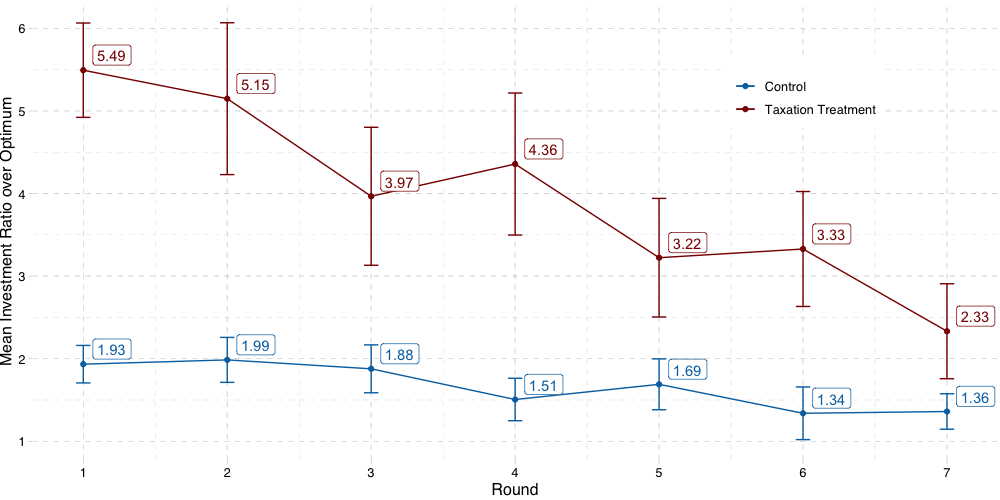
\includegraphics[width=\textwidth]{graphs/over_invest.png}
    \caption{Ratio of Over Investment per Round}
    \label{fig:over_invest}
\end{figure}

Table \ref{tab:over_invest} present a linear mixed model dissecting the most important effects on over investing. The random effects are \textit{participant, group} and \textit{gender}.

\begin{table}[!htbp] \centering 
  \caption{Linear Mixed Model Over Investment Ratio} 
  \label{tab:over_invest} 
\begin{tabular}{@{\extracolsep{5pt}}lcc} 
\\[-1.8ex]\hline 
\hline \\[-1.8ex] 
\\[-1.8ex] & \multicolumn{2}{c}{Ratio of Investment Over Optimum} \\ 
\\[-1.8ex] & (1) & (2)\\ 
\hline \\[-1.8ex] 
 Treatment(True) & 2.314$^{***}$ & 2.049$^{***}$ \\ 
  & (0.698) & (0.678) \\ 
  & & \\ 
 Round & $-$0.307$^{***}$ & $-$0.307$^{***}$ \\ 
  & (0.055) & (0.055) \\ 
  & & \\ 
 Was Winner in Previous & 0.256 & 0.283 \\ 
  & (0.271) & (0.271) \\ 
  & & \\ 
 CRT Score &  & $-$0.157 \\ 
  &  & (0.283) \\ 
  & & \\ 
 MPL &  & $-$0.371$^{***}$ \\ 
  &  & (0.125) \\ 
  & & \\ 
 Constant & 2.813$^{***}$ & 5.737$^{***}$ \\ 
  & (0.546) & (1.088) \\ 
  & & \\ 
Observations & 672 & 672 \\ 
Log Likelihood & $-$1,751.726 & $-$1,748.247 \\ 
Akaike Inf. Crit. & 3,519.453 & 3,516.495 \\ 
Bayesian Inf. Crit. & 3,555.535 & 3,561.597 \\ 
\hline \\[-1.8ex] 
\textit{Notes:} & \multicolumn{2}{l}{$^{***}$Significant at the 1 percent level.} \\ 
 & \multicolumn{2}{l}{$^{**}$Significant at the 5 percent level.} \\ 
 & \multicolumn{2}{l}{$^{*}$Significant at the 10 percent level.} \\ 
\end{tabular} 
\end{table} 